\documentclass{article}

\textwidth=6.5in
\textheight=8.5in
\voffset=-54pt
\oddsidemargin=0in
\evensidemargin=0in
\setlength{\parskip}{8pt}
\setlength{\parindent}{0pt}

\usepackage{workbook}

\usepackage{handout}

\usepackage{exam}

\newcommand{\answerbox}[3][]{
    \fbox{\begin{minipage}[t][#2][c]{#3}
        #1
    \end{minipage}}
    }

\begin{document}

\probonly{
\begin{center}
  \large\textsc{Final Exam Practice 4}
  
      \pspace{12pt}
  \begin{problemonly}\large Name: \rule{5cm}{0.15mm}\\ \end{problemonly}
\end{center}

\emph{This exam reflection and the attached practice exam will be due on Monday, May 5th, at the same time your problem sets were due during the semester. The grading will be based on completion and genuine effort.}

\begin{enumerate}
    \item Follow these directions while doing the practice exam. Attempt each problem without any aids. In the left-hand margin next to each part, record how long you spent on the problem and whether you 
    \begin{enumerate}[label=\Alph*.,nosep]
        \item were able to complete the problem on your own
        \item got stuck partway
        \item didn't know how to start
    \end{enumerate}
    \textbf{After attempting the problems without any aids,} pull up the solutions on Canvas and use them to help you answer the following questions.

    \item List the problems/parts that you didn't know how to start. For each, skim the solutions and write down the topics involved that you need to review. (Use the workbook's table of contents as a guide.) You should return to these problems after you review those topics. (OH and MQC are good for this.)

    \pspace{\vfill}
    
    \item List the problems/parts on which you got stuck partway. Read the solutions one line at a time until you find where you went wrong or got stuck. What were the key ideas or skills involved that you need to practice for the actual exam? You should put the solutions away and retry the problem yourself.
    \pspace{\vfill}

    \pspace{\newpage}

    \item 
    List the problems you were able to complete on your own. For each, compare your work to the solutions. Be strict. If you made any mistakes, try to categorize them. Did you make an algebra mistake? A differentiation mistake? Did you misunderstand the problem? Was your strategy wrong? How do you plan to not make the same mistake on the actual exam? For extra practice, redo the problem.

    \pspace{\vfill}
    
    \item You will have three hours for the final exam. Imagine that you were taking the exam today. Based on how well you were able to do these problems on your own and how long they took you, what grade do you think you would earn? If you aren't satisfied with this grade, what specific actions to you intend to take between now and May 12th?

    \pspace{\vfill}

\end{enumerate}

\newpage
}

\setcounter{page}{1}

{\large \mbox{} \hfill \bf Name:\underline{\hspace{3in}}}\\[2pt]
{\mbox{} \hfill \it (Please write your name neatly in print.)}\\[12pt]
{\large \mbox{} \hfill \bf HUID:\underline{\hspace{3in}}}
 
\medskip
 
\noindent
{\large\bf
Final Exam Practice 4\\
Math Mb Spring 2025}
\noindent


{\Large
\begin{center}\textbf{Directions---Please read carefully!} \end{center}}

This is a practice test. The same directions will appear on the actual exam, so read them carefully.

\hrulefill 


This exam is subject to the Harvard College Honor Code. No calculators or any other aids are permitted.  Please write as neatly as possible, as answers that can't be read can't be graded and thus can't receive credit. To receive full credit, you must show relevant working
and include units when appropriate. 

You have 180 minutes to complete this exam. 

You may ask for scratch paper if you need additional space to write, but it will not be scanned or graded. Make sure to include all relevant working in this exam booklet in the space provided for each question.

\begin{center}\textbf{Good luck!}\end{center}


\vfill

\centering{
\emph{As a member of Harvard College, I pledge that I will not give or receive assistance on this exam.}}
\vspace{0.3in}

{\large \mbox{} \hfill \bf Signature:\underline{\hspace{3in}}}
\thispagestyle{empty}

\newpage

\begin{enumerate}

\item

\begin{grading}
    3/2/2
\end{grading}

 Belle Isle Inlet is an urban nature preserve in Suffolk County, MA. At the entrance of the preserve, the height of the tide (in feet) is recorded throughout the day, and the measurements are graphed below. We can model this with a sinusoidal function $B(t)$, where $t$ is time after 5am. 

        \begin{center}
          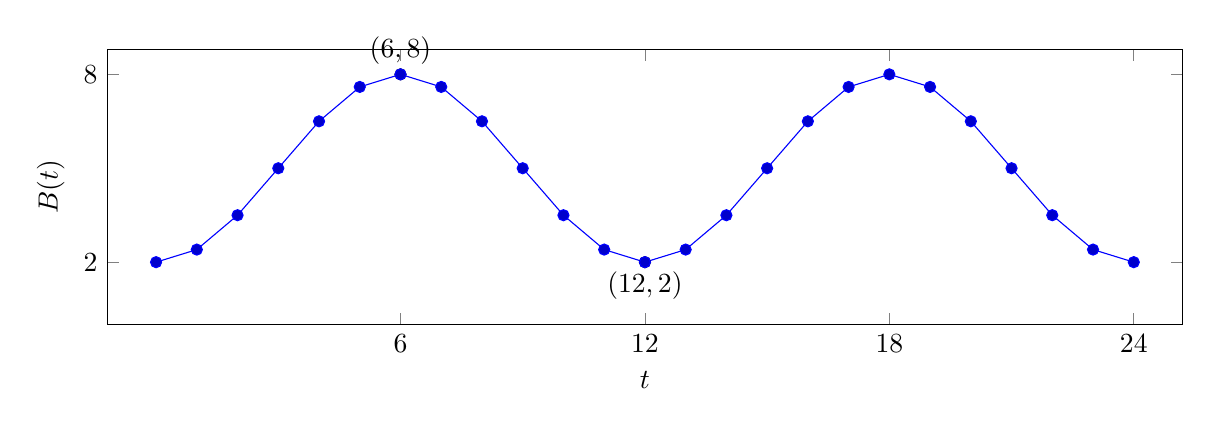
\begin{tikzpicture}
            \begin{axis}[xtick={6, 12, 18, 24},
            xticklabels={$6$, $12$, $18$, $24$}, 
            ytick={2, 8}, xlabel=$t$, ylabel=$B(t)$,
            width=6in, height=2in, enlarge x limits=0.05, 
            ymin = 0, clip=false]
              \addplot+[domain=0:24] {-3*cos(pi/6*deg(x))+5};
              %\addplot+[domain=0:25, dashed, black] {50};
              \filldraw (6,8) circle[radius=2pt] (12,2) circle[radius=2pt];
              \node[above] at (6,8) {$(6,8)$};
              \node[below] at (12,2) {$(12,2)$};
            \end{axis}
          \end{tikzpicture}
        \end{center}


\begin{enumerate}
    \item 
    \begin{problem}
    Find the amplitude, midline value, and period of $B(t)$.
    \end{problem}
\pspace{1.5in}

\begin{solution}
The amplitude of a sinusoid is the amount by which the output oscillates above and below the midline value. The midline value is half-way between the maximum and minimum output values. The period is the input interval required for a full cycle.
    \begin{itemize}
        \item $\text{amplitude} = \dfrac{\text{max} - \text{min}}{2} = \boxed{3}$
        \item $\text{midline value} = \dfrac{\text{max} + \text{min}}{2} = \boxed{5}$
        \item $\text{period} = \boxed{12}$
    \end{itemize}
\end{solution}

    \probonly{
    Amplitude = \hrulefill \hfill Midline Value = \hrulefill \hfill Period = \hrulefill
    }
    
    \item 
    \begin{problem}
    Write a formula for $B(t)$. 
    \end{problem}
    \pspace{0.75in} 

    \begin{solution}
        Since the minimum value of the function occurs at $t=0$, we can come up with the formula for $B(t)$ by starting with $-\cos(t)$ and we will not have to use a phase shift. We need to multiply the outputs by $3$ and add $5$ to achieve the correct amplitude and midline value. We need to convert a period of $12$ hours into $2\pi$ radians, so we should multiply the inputs by $\frac{\pi}{6}$. This gives us \fbox{$B(t)=-3\cos(\frac{\pi}{6}t)+5$.}
    \end{solution}

    \item  
    \begin{problem}
    When is the tide 7 feet high for the first time after 5am? Give an exact answer in terms of inverse trig functions.
    \end{problem}
    \pspace{4in}

    \begin{solution}
        $B(t)$ models the tide height in feet where $t$ is the number of hours after 5am, so we need to find the first solution after $t=0$ to $B(t)=7$.
        \begin{align*}
            -3\cos(\tfrac{\pi}{6}t)+5 &= 7\\
            \cos(\tfrac{\pi}{6}t) &= -\tfrac{2}{3}
            \intertext{The first solution to this equation after $t=0$ is when}
            \tfrac{\pi}{6}t &= \arccos(-\tfrac{2}{3})\\
            t &= \tfrac{6}{\pi}\arccos(-\tfrac{2}{3})
        \end{align*}
        The tide will be 7 feet high \fbox{$\tfrac{6}{\pi}\arccos(-\tfrac{2}{3})$ hours after 5am.} (Or $6-\tfrac{6}{\pi}\arccos(\tfrac{2}{3})$ hours after 5am.)
    \end{solution}

    %     \begin{feedback}
    %     Leave your feedback here:
    %     KP: This took 4:02. The decimal values felt like a weird move for us and were an unnecessary complication, especially at the end. Consider changing the values.
    %     MK: I agree that we should use integer values.
  
    % \end{feedback}
        
\end{enumerate}

\newpage 


\item 

    \begin{grading}
        Part (a) - 2/3/3, Part (b) - 1/2
    \end{grading}

\begin{enumerate}
    \item  
    \begin{problem}
    Compute the derivatives of the following functions.
    \end{problem}

    \begin{enumerate} 
        
        \item 
        \begin{problem}
        $g(x)=\arcsin(e^x)$
        \end{problem}
        \pspace{\vfill}

        \begin{solution}
            \begin{align*}
                g'(x) &= \diff*{\arcsin(e^x)}{x} \\
                &= \frac{1}{\sqrt{1-(e^x)^2}} \cdot \diff*{e^x}{x} \\
                &= \frac{1}{\sqrt{1-e^{2x}}} \cdot e^x \\
                &= \boxed{\frac{e^x}{\sqrt{1-e^{2x}}}}
            \end{align*}
        \end{solution}

        \item 
        \begin{problem}
        $f(x)=\ln(1+\sqrt{x^2+1})$
        \end{problem}
        \pspace{\vfill}

        \begin{solution}
            \begin{align*}
                f'(x) &= \diff*{\ln(1+\sqrt{x^2+1})}{x} \\
                &= \frac{1}{1+\sqrt{x^2+1}} \cdot \diff*{(1+\sqrt{x^2+1})}{x} \\
                &= \frac{1}{1+\sqrt{x^2+1}} \cdot \tfrac{1}{2}(x^2+1)^{-1/2} \cdot \diff*{(x^2+1)}{x} \\
                &= \frac{1}{1+\sqrt{x^2+1}} \cdot \tfrac{1}{2}(x^2+1)^{-1/2} \cdot 2x \\
                &= \boxed{\frac{x}{x^2+1+\sqrt{x^2+1}}}
            \end{align*}
        \end{solution}
    
        
        \item 
        \begin{problem}
            $j(x)=(\cos x)^{2x}$
        \end{problem}
        \pspace{\vfill}

        \begin{solution}
            This is a function of the form $f(x)^{g(x)}$, so we can use logarithmic differentiation. 

            \begin{align*}
                j(x) &= (\cos x)^{2x} \\
                \ln j(x) &= \ln\!\big[(\cos x)^{2x}\big] \\
                 &= 2x\ln(\cos x)
                \intertext{
                Differentiating both sides,
                }
                \frac{j'(x)}{j(x)} &= 2\ln(\cos x) - \frac{2x\sin x}{\cos x} \\
                j'(x) &= j(x)\Big[2\ln(\cos x) - \frac{2x\sin x}{\cos x}\Big] \\
                &= \boxed{2(\cos x)^{2x}\big[\ln(\cos x) - x\tan x\big]}
            \end{align*}
        \end{solution}
    \end{enumerate}
    
\newpage
        \item Consider the function $h(x)=\displaystyle \int_{1}^{x} \cos(t^2) \, dt$. 
        
        \begin{enumerate}
            \item 
            \begin{problem}
            Find $h'(x)$.
            \end{problem}
            \pspace{\vfill}

            \begin{solution}
                By Part 1 of the Fundamental Theorem of Calculus, $h'(x) = \boxed{\cos(x^2)}$.
            \end{solution}
            
            \item 
            \begin{problem}
            Find $h'\!\left(\sqrt{\frac{\pi}{6}}\,\right)$. Simplify completely.
            \end{problem}
            \pspace{\stretch{2}}

            \begin{solution}
                $h'(\sqrt{\frac{\pi}{6}}) = \cos \frac{\pi}{6} = \boxed{\tfrac{\sqrt{3}}{2}}$.
            \end{solution}
        \end{enumerate}
    \end{enumerate}
    
    % \item Consider the implicit curve defined by 
    % \begin{center}
    %     $xy+y^2=y^4$.
    % \end{center}
    % Find $\dfrac{dy}{dx}$ at the point $(0,1)$.
    % \vfill\vfill\vfill
    
    % \newpage
    % \item Evaluate the following integrals. 
    % \begin{enumerate}
    %     \item $\displaystyle \int_{1}^{e} \dfrac{\ln x}{x} \, dx$
    %     \vfill
    %     \item $\displaystyle \int x\ln x\, dx$
    %     \vfill
    % \end{enumerate}
    % \end{enumerate}

    %\begin{feedback}
    %    Leave your feedback here:
     %   KP: This took 2:44.
     %   MK: Maybe here we can add one integration by substitution, one integration by parts.
   % \end{feedback}


\pspace{\newpage}





\item
\begin{grading}
    3/1/1/2/2
\end{grading}

\begin{problem}
 A hiker begins hiking at a time designated as $t=0$; her elevation at the start of the hike is 70 meters. The function $f(t)$ models the \textbf{the rate of change of a hiker's elevation} in meters per hour $t$ hours after the start of a 7 hour hike. The graph of $f(t)$ is shown below.
\end{problem}
 

  \newcommand{\graph}{
      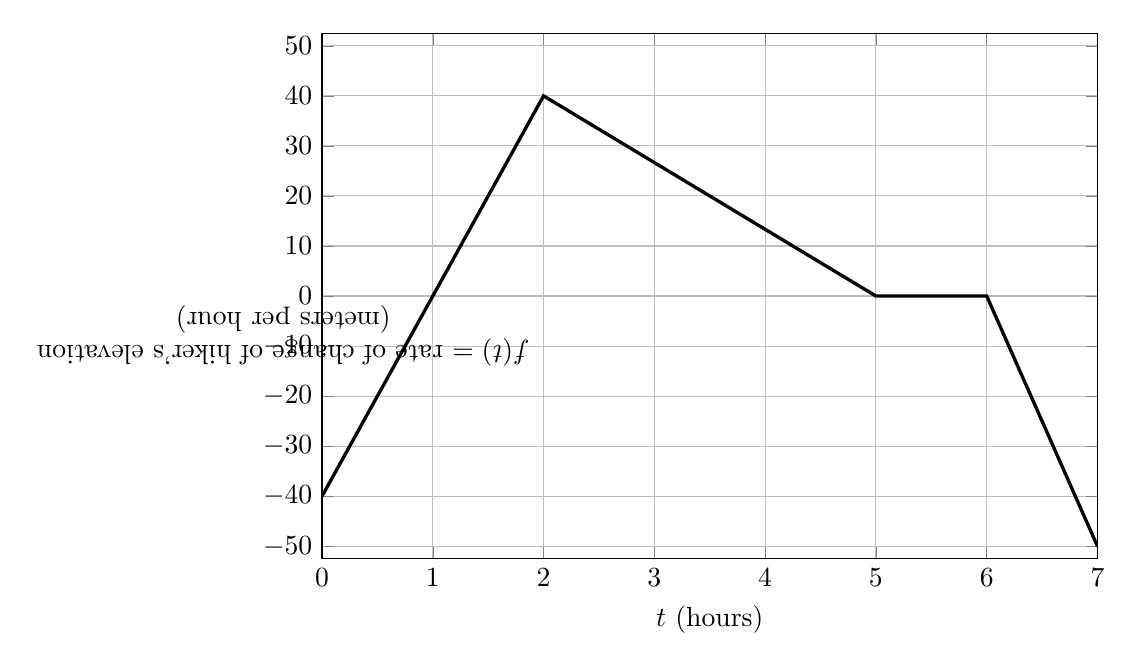
\begin{tikzpicture}
        \begin{axis}[
        xlabel = $t$ (hours),
        ylabel = {$f(t) =$ rate of change of hiker's elevation \\
        (meters per hour)},
        ylabel style = {align=center,
            at={(axis description cs:-0.05,.5)},anchor=south, rotate=90},
        xmin = 0, xmax = 7,
        ymin = -52.5, ymax = 52.5,
        ytick distance = 10,
        width = 4.5in,
        height = 3.25in,
        grid = major,
        ]
        \coordinate (A) at (0,-40);
        \coordinate (B) at (2,40);
        \coordinate (C) at (5,0);
        \coordinate (D) at (6,0);
        \coordinate (E) at (7,-50);
        % \coordinate (F) at (7.5,-50);
        \draw[very thick] (A) -- (B) -- (C) -- (D) -- (E);
        \addplot[draw=none]{0};
        \end{axis}
      \end{tikzpicture}
    }
    \graph

    
    \begin{enumerate}

    \item
    \begin{enumerate}
        \item 
        \begin{problem}
        On what interval(s) on $[0,\,7]$ is the hiker's elevation increasing?
        \end{problem}
        \pspace{0.5in}

        \begin{solution}
            The hiker's elevation is increasing on the interval $[1, 5]$ since the rate of change of her elevation is positive on $(1, 5)$ and the hiker's elevation is a continuous function of time.

            Alternative answer: The hiker's elevation is increasing on the interval $(1, 5)$ since $f(t)$ is positive on this interval.
        \end{solution}

        
        \item 
        \begin{problem}
        On what interval(s) on $[0,\,7]$ is the hiker's elevation decreasing?
        \end{problem}
        \pspace{0.5in}

        \begin{solution}
            The hiker's elevation is decreasing on the intervals $[0, 1]$ and $[6, 7]$ since the rate of change of her elevation is negative on $(0, 1)$ and $(6, 7)$ and the hiker's elevation is continuous.

            Alternative answer: The hiker's elevation is decreasing on the intervals $(0, 1)$ and $(6, 7)$ since $f(t)$ is negative on these intervals.
        \end{solution}

        \item 
        \begin{problem}
        On what intervals(s) on $[0,\,7]$ is the hiker's elevation constant?
        \end{problem}
        \pspace{0.5in}

        \begin{solution}
            The hiker's elevation is constant on the interval $[5, 6]$ since the rate of change of her elevation is zero on $[5, 6]$.
        \end{solution}

    \end{enumerate}

\item 
\begin{problem}
At what time(s) or on what time interval(s) is the hiker at her highest elevation?
\end{problem}
\pspace{0.5in}

\begin{solution}
Since the hiker's elevation decreases from $t=0$ to $t=1$, increases from $t=1$ to $t=5$, is constant from $t=5$ to $t=6$, then decreases from $t=6$ to $t=7$, her maximum elevation could occur at either $t=0$ or on the interval $[5, 6]$. We are told that the hiker's elevation at $t=0$ is $70$ meters. The hiker's elevation on $[5, 6]$ is $70+\int_0^5 f(t)\,dt$ meters. Based on the graph, this $\int_0^5 f(t)\,dt$ is positive, so the maximum height occurs on the time interval $[5, 6]$. 
\end{solution}

\item
\begin{problem}
What is the hiker's maximum elevation throughout the 7 hour hike? Simplify completely.
\end{problem}
\pspace{2in}
      
\begin{solution}
    The hiker's maximum elevation occurs on the time interval $[5, 6]$ and is $70+\int_0^5 f(t)\,dt$ meters. Using the graph, $\int_0^5 f(t)\,dt=60$ meters, so the hiker's maximum elevation is \fbox{$130$ meters.}
\end{solution}

\pspace{\newpage} 

\probonly{
\textit{(Continued from previous page)}

        \graph
}

\item  
\begin{problem}
What is the hiker's elevation at time $t=7$? Simplify completely.
\end{problem}
\pspace{\vfill} 

\begin{solution}
    The hiker's elevation at time $t=7$ is $130+\int_6^7 f(t)\,dt$ meters. Using the graph, $\int_6^7 f(t)\,dt =-25$ meters, so the hiker's elevation at time $t=7$ is \fbox{$105$ meters.}
\end{solution}

\item 
\begin{problem}
How many time(s) after $t=0$ will the hiker be at the same elevation as when she started? At what time(s) does this happen? Write 1-2 sentences explaining your reasoning.
\end{problem}
\pspace{\stretch{2}}

\begin{solution}
    The hiker's elevation at time $t$ is $70+\int_0^t f(\tau)\,d\tau$ meters, so the hiker's elevation will be the same as when she started when $\int_0^t f(\tau)\,d\tau=0$. Using the graph, this occurs only at $t=2$.
\end{solution}

\end{enumerate}

%     \begin{feedback}
%         Leave your feedback here:
% KP: This took 6:54. Asking for explanation so frequently made the time on this question swell substantially and was extremely tedious. I don't think it is worth the time increase to read explanations that are so similar to each other. I'm not sure this should be worth 17/90 points as a topic to begin with, trimming that down and asking for explanation more sparingly could tighten time. For example it felt tedious to be asking for explanation for b and c. I think making the prompt "make it clear what you are calculating to receive full or partial credit." would allow us to grade reasonably. I think removing e entirely would be a good move for length.

% MK: I'm on board with getting rid of all the explanation components of the questions and (e). If this feels extreme, I think (b) and (c) have explanations that are straightforward, so I'd be okay keeping these.
%     \end{feedback}

\pspace{\newpage}

\item

\begin{grading}
    6/6
\end{grading}

\begin{problem}
 Two boats set sail at the same time from a dock. Boat $A$ is headed directly east of the dock at a speed of 2.5 miles per hour and Boat $B$ is headed directly south of the dock at a speed of 6 miles per hour.
 \end{problem}
 
\begin{enumerate}
    \item  
\begin{problem}
At what rate, in miles per hour, is the distance between the two boats changing after 2 hours?
\end{problem}
\pspace{\vfill}

\begin{solution}
    This is a related rates problem. We should draw a snapshot picture after 2 hours and a generic picture representing a generic time $t$.

\begin{center}
\begin{tabular}{cc}
\textbf{Snapshot} & \textbf{Generic} \\[6pt]
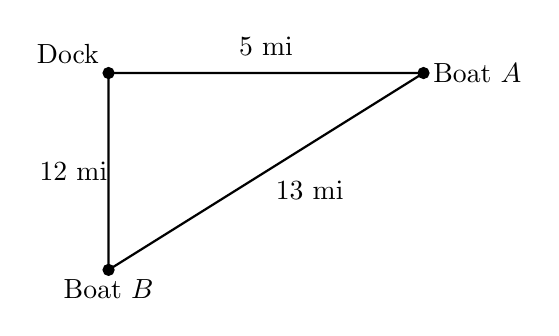
\begin{tikzpicture}
\filldraw (0,0) circle (2pt) node[above left] {Dock};
\filldraw (4,0) circle (2pt) node[right] {Boat $A$};
\filldraw (0,-2.5) circle (2pt) node[below] {Boat $B$};
\draw[thick] (0,0) -- (4,0) -- (0,-2.5) -- cycle;

\node[above] at (2,0.1) {$5$ mi};
\node[right] at (-1,-1.25) {$12$ mi};
\node[below right] at (2, -1.25) {$13$ mi};
\end{tikzpicture}
&
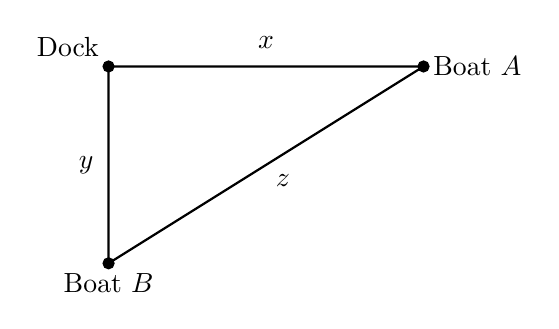
\begin{tikzpicture}
\filldraw (0,0) circle (2pt) node[above left] {Dock};
\filldraw (4,0) circle (2pt) node[right] {Boat $A$};
\filldraw (0,-2.5) circle (2pt) node[below] {Boat $B$};
\draw[thick] (0,0) -- (4,0) -- (0,-2.5) -- cycle;

\node[above] at (2,0.1) {$x$};
\node[right] at (-0.5,-1.25) {$y$};
\node[below right] at (2, -1.25) {$z$};
\end{tikzpicture}
\end{tabular}
\end{center}

We are given in the problem that $\diff{x}{t} = 2.5$ mph and $\diff{y}{t}=6$ mph. We want to find $\diff{z}{t}$. We can write down a relationship between the variables using the Pythagorean Theorem.
\begin{align*}
    x^2+y^2&=z^2
    \intertext{Now we can differentiate both sides with respect to $t$.}
    2x\diff{x}{t}+2y\diff{y}{t} &= 2z\diff{z}{t}
    \intertext{Now we can plug in the rates and the snapshot information at $t=2$.}
    2(5\text{ mi})(2.5\text{ mph}) + 2(12\text{ mi})(6\text{ mph}) &= 2(13\text{ mi})\diff{z}{t}
    \end{align*}
    Solving for $\diff{z}{t}$, we find
    \begin{align*}
    \diff{z}{t} &= \frac{2(5\text{ mi})(2.5\text{ mph}) + 2(12\text{ mi})(6\text{ mph})}{2(13\text{ mi})} \\
    &= \boxed{6.5 \text{ mph}}
\end{align*}

\end{solution}

\item  
\begin{problem}
After 2 hours pass, Boat $A$ \underline{stops moving} to take some measurements with two telescopes: one that faces back towards the dock and one that tracks Boat $B$ as it continues to move south at 6 miles per hour. At what rate, in radians per hour, is the angle between the two telescopes' lines of sight changing at this moment?
\end{problem}
\pspace{\vfill}

\begin{solution}
Let's draw diagrams again.

\begin{center}
\begin{tabular}{cc}
\textbf{Snapshot} & \textbf{Generic} \\[6pt]
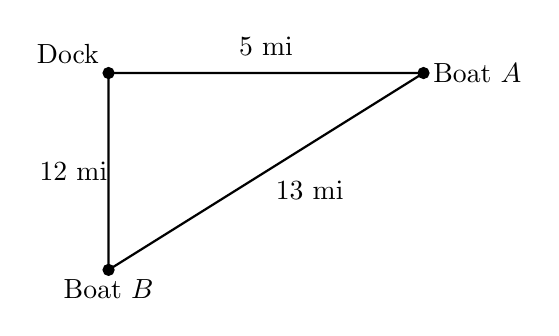
\begin{tikzpicture}
\filldraw (0,0) circle (2pt) node[above left] {Dock};
\filldraw (4,0) circle (2pt) node[right] {Boat $A$};
\filldraw (0,-2.5) circle (2pt) node[below] {Boat $B$};
\draw[thick] (0,0) -- (4,0) -- (0,-2.5) -- cycle;

\node[above] at (2,0.1) {$5$ mi};
\node[right] at (-1,-1.25) {$12$ mi};
\node[below right] at (2, -1.25) {$13$ mi};
\end{tikzpicture}
&
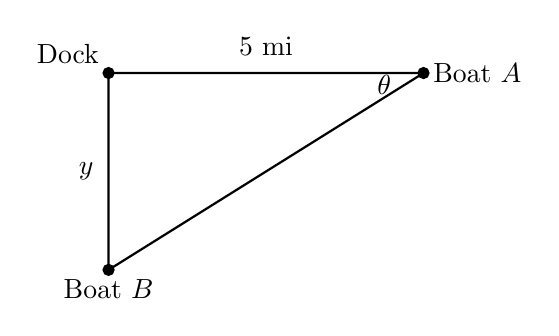
\begin{tikzpicture}
\filldraw (0,0) circle (2pt) node[above left] {Dock};
\filldraw (4,0) circle (2pt) node[right] {Boat $A$};
\filldraw (0,-2.5) circle (2pt) node[below] {Boat $B$};
\draw[thick] (0,0) -- (4,0) -- (0,-2.5) -- cycle;

\node[above] at (2,0.1) {$5$ mi};
\node[right] at (-0.5,-1.25) {$y$};
\node at (3.5,-0.15) {$\theta$};
\end{tikzpicture}
\end{tabular}
\end{center}

We are given $\diff{y}{t}=6$ mph, and we want to find $\diff{\theta}{t}$. We can write down a relationship between the variables using trigonometric functions.
\begin{align*}
    \tan \theta &= \frac{y}{5}
    \intertext{Differentiating both sides with respect to $t$,}
    \sec^2(\theta) \diff{\theta}{t} &= \frac{1}{5} \diff{y}{t}
    \intertext{We can find $\sec^2(\theta)$ at $t=2$ using our snapshot diagram and remembering that $\sec \theta $ is the ratio of the hypotenuse to the adjacent side. Plugging in the information at $t=2$,}
    \Big(\frac{13}{5}\Big)^{\!2} \diff{\theta}{t} &= \frac{1}{5}(6) \\[6pt]
    \diff{\theta}{t} &= \boxed{\frac{30}{169} \text{ rad/s}}
\end{align*}

\end{solution}

\end{enumerate}

\pspace{\newpage}

    % \begin{feedback}
    % Leave your feedback here:

    % (MS) I would add another bullet point which says "include the unit in your final answer." I understand that this should be an expectation; at the same time, I can also see how this can be considered as assumed. \textit{("But the problem is talking about miles and hours; what else would it be?")} Since we are already instructing them through the bullet points, setting expectations on the answer format, I would consider adding this one, as well.\\ 

    % KP: a took 3:21 and b took 4:03. We have inconsistently required two diagrams and it feels like not the time to start. I think asking for one diagram and clearly labeling any introduced variables would be ample instruction. I agree with units in final answer suggestion from Mario.

    % MK: Yeah, I feel like often times our rubrics on exams for related rates do not give much or any credit for writing goal/known or having the pictures...we usually start giving credit for the model, right? Maybe we can frame these as recommendations or reminders for how we solved these problems formally in section.

    % Maybe also bold and rephrase "Boat x sails for two hours then stops moving so the boat can take stationary measurements" or something of the like. 
    % \end{feedback}

\item 

\begin{grading}
    1/1/1/2
\end{grading}

\begin{problem}
An oil spill forms a large circular puddle on the ground. The radius of the puddle is 20 meters. 
\end{problem}

\begin{enumerate} 

\item 
\begin{problem}
Assume the density of oil throughout the puddle is a constant 5 $\text{g/m}^2$. Calculate the total amount of oil (in grams) in the entire puddle.
\end{problem}
\pspace{\vfill}

\begin{solution}
    The total amount of oil will be the area of the puddle multiplied by the area density of the oil. The area of the puddle is $\pi (20\,\text{m})^2 = 400\pi\,\text{m}^2$. So the total amount of oil in the puddle is $(400\pi\,\text{m}^2)(5\,\text{g/m}^2)=\boxed{2000\pi\,\text{g}}$.
\end{solution}
 

\item 

\begin{problem}
Suppose instead that the density of oil changes depending on the distance $x$ (in meters) from the middle of the puddle. The density is given by $\rho(x) \text{ g/m}^2$. We want to find the total amount of oil (in grams) in the entire puddle under this assumption.

 Which of these best describes the way you would slice the region (into $n$ slices) as a first step to arriving at an integral? \probonly{Circle your choice.

 \begin{enumerate}
     \item concentric circular rings
     \item horizontal strips
     \item vertical strips
 \end{enumerate}}
 \end{problem}

 \begin{solution}
     The best way to slice the region is into \fbox{concentric circular rings,} because the density varies with the distance from the center of the puddle, and so the density will be approximately constant on a circular ring.
 \end{solution}
 %\item Given your choice in (b),  define what $\Delta x$ and $x_k$ would be in this scenario (with $n$-slices).\\
 %\vfill
 %$\Delta x$ = \hrulefill \hfill $x_k$ = \hrulefill \hfill 
 \item 
 \begin{problem}
 Which of the following sums is a good approximation of the total amount of oil (in grams) in the entire puddle? \probonly{Circle your choice.
\begin{enumerate}
     \item $\displaystyle \sum_{k=1}^n \rho(x_k) \cdot 20 \Delta x$
     \item $\displaystyle \sum_{k=1}^n\rho(x_k) \cdot 40 \Delta x$
     \item $\displaystyle \sum_{k=1}^n\rho(x_k) \cdot \pi x_k^2 \Delta x$
     \item $\displaystyle \sum_{k=1}^n\rho(x_k) \cdot 2\pi x_k \Delta x$
     \item $ \displaystyle \sum_{k=1}^n\rho(x_k) \cdot 4\cdot\sqrt{400-x_k^2}\;\Delta x$
 \end{enumerate}}
 \end{problem}

 \begin{solution}
 The amount of oil in the $k$th circular ring will be the density $\rho(x_k)$ times the area $2\pi x_k\Delta x$, so the correct sum is \fbox{$\displaystyle \sum_{k=1}^n\rho(x_k) \cdot 2\pi x_k \Delta x$.}
 \end{solution}

 \item 
 \begin{problem}
 Let $\displaystyle \rho(x) = \frac{5}{x^2 + 20} \text{ g/m}^2$. Write an integral that represents the total amount of oil (in grams) in the entire puddle. You do not need to evaluate it.
 \end{problem}
 \pspace{\vfill}

 \begin{solution}
     $\displaystyle \int_0^{20} \frac{5}{x^2+20}\cdot 2\pi x\,dx$
 \end{solution}

 \end{enumerate}

 

 %    \begin{feedback}
 %        Leave your feedback here. 

 % (MS) I got confused and completely stuck because I was modeling the oil inside the pipe and not the spilled one on the floor. I plotted a pipe leaking and, thinking of the oil density, I was slicing the oil in the pipe. Looking back, I can see that the text does talk about the oil spill (I see that word appearing three times until the end of the problem (a).

 % I feel that my blunder is coming from getting used to slicing liquids contained in a certain closed frame (in this case, a pipe). My concern is that this may happen to some more people in the exam, resulting to a close-to-zero score out of a significant number of points assigned to this problem.

 % I would suggest stressing out the spill even more. Perhaps a sentence before (a) that says "In this problem, let us analyze the quantity of the spilled oil on the floor that forms the shape of a circle." I think it is good to additionally stress the circular shape of the spill as it isn't quite obvious this should be the case (perhaps in the ideal physical conditions and the floor design).

 % There are also a few phrases I would consider rephrasing.
 % \begin{itemize}
 %     \item I would remove "Complete the following $3$ multiple choice questions." This sentence is redundant and incorrect (there are $2$ such problems and they aren't "the following" as they begin from (b)).
 %     \item I would rephrase "number of grams" in (a) into "the amount in grams". The phrase is a bit unusual to me, if not (incorrectly) implying that an integer is expected for an answer.
 %     \item I would change "Which picture" to "Which of these" -- there are no pictures given.
 % \end{itemize}
 % KP This took 2:57, but the language needs to be significantly clarified. Part a in particular mentions within 30 m of the center so often that it's confusing. Restructure. "Assume the density of oil was. . ." I would put a value there. Addition another constant letter seems like it is unnecessarily confusing when what we want is this to be an accessible computation of mass (b) I would remove the comment about being realistic. "Now assume the density of oil instead varies with distance from the center of the spill..."
 %    \end{feedback}

\pspace{\newpage }


 \item 
 \begin{problem}
 Consider the implicit curve defined by 
    \begin{center}
        $xy+y^2=y^4$.
    \end{center}
    Find $\dfrac{dy}{dx}$ at the point $(0, 1)$.
  \end{problem}
  \pspace{\vfill}

\begin{solution}
To find $\diff{y}{x}$, we should use implicit differentiation and differentiate with respect to $x$.
\begin{align*}
    \diff*{xy+y^2}{x} &= \diff*{y^4}{x} \\[4pt]
    \diff*{xy}{x} + \diff*{y^2}{x} &= \diff*{y^4}{x} \\[4pt]
    \Big(y+x\diff{y}{x}\Big) + 2y\diff{y}{x} &= 4y^2\diff{y}{x}
    \intertext{Since we want $\diff{y}{x}$ at $(0, 1)$, we can plug these values in.}
    \Big((1)+(0)\diff{y}{x}\Big) + 2(1)\diff{y}{x} &= 4(1)^2\diff{y}{x} \\[4pt]
    1+2\diff{y}{x}&= 4\diff{y}{x} \\[4pt]
    1 &= 2\diff{y}{x} \\
    \boxed{\frac{1}{2}} &= \diff{y}{x}
\end{align*}
\end{solution}

\pspace{\newpage}
    
    \item 

    \begin{grading}
        3/3
    \end{grading}

    \begin{problem}
    Evaluate the following integrals.
    \end{problem}
    
    \begin{enumerate}
        \item 
        \begin{problem}
        $\displaystyle \int_{1}^{e} \dfrac{\ln x}{x} \, dx$
        \end{problem}
        \pspace{\vfill}

        \begin{solution}
            We can use integration by substitution. Let $u=\ln x$, and so $du = \tfrac{1}{x}\,dx$.
            \begin{align*}
                \int_{1}^{e} \dfrac{\ln x}{x} \, dx &= \int_0^1 u\,du \\
                &= \tfrac{1}{2}\big[u^2\big]_0^1\\
                &= \boxed{\frac{1}{2}}
            \end{align*}
        \end{solution}
        
        \item 
        \begin{problem}
        $\displaystyle \int x\ln x\, dx$
        \end{problem}
        \pspace{\vfill}

        \begin{solution}
            We can use integration by parts. Let $u=\ln x$, $dv = x\,dx$, so $du = \tfrac{1}{x}\,dx$, $v=\frac{1}{2}x^2$.

            \begin{align*}
                \int x\ln x\, dx &= \frac{1}{2}x^2\ln x - \int\frac{1}{2}x^2\cdot \frac{1}{x}\,dx\\
                &= \frac{1}{2}x^2\ln x - \frac{1}{2}\int x\,dx \\
                &= \boxed{\frac{1}{2}x^2\ln x - \frac{1}{4}x^2 + C}
            \end{align*}
        \end{solution}
    \end{enumerate}

\pspace{\newpage}
 
\item 

\begin{grading}
    4/2
\end{grading}

\begin{problem}
The shaded region below is bounded by the graphs of
$x=y^2$ and $y=x-2$. 
\end{problem}

\begin{center}
    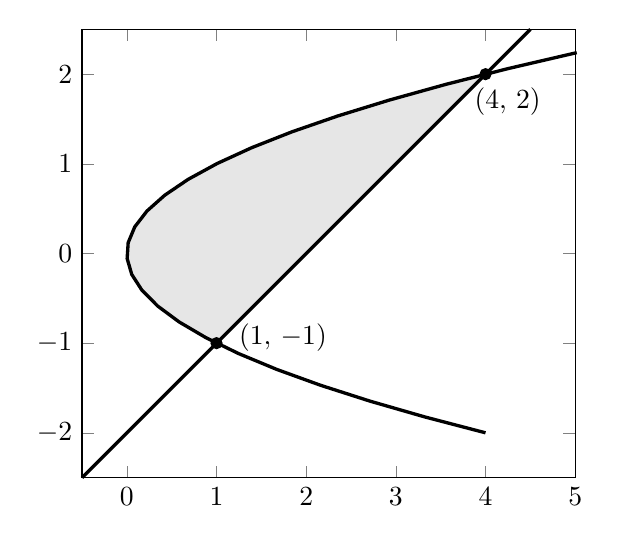
\begin{tikzpicture} 
      \begin{axis}[cycle list={black}, xmin=-0.5, xmax=5,
      ymin=-2.5, ymax=2.5,
        axis equal image, clip=false] 
        \fill[gray, opacity=0.2] plot[domain=-1:2] (\x*\x,\x) -- plot[domain=-1:2] ({\x+2},\x);
        \addplot+[very thick, domain=-2:2.24] (x^2,x);
        \addplot+[very thick, domain=-2.5:2.5] (x+2, x);
        \filldraw (1,-1) circle[radius=2pt] (4,2) circle[radius=2pt];
        \node[xshift=24pt, yshift=2pt] at (1,-1) {$(1,\,{-1})$};
        \node[xshift=8pt, yshift=-10pt] at (4,2) {$(4,\,2)$};
      \end{axis} 
    \end{tikzpicture}

\end{center}

\begin{enumerate}
    \item 
    \begin{problem}
    Write, but do not evaluate, a definite integral that would give the area
    of the shaded region. \textit{(One direction of slicing may be more efficient than others!)}
    \end{problem}
    \pspace{\vfill}

    \begin{solution}
        Since right and left boundaries of the region are given by single curves ($x=y+2$ and $x=y^2$ respectively,) it will be easier for us to slice horizontally. The area of the $k$th slice is $(y_k+2 -y_k^2)\Delta y$, which leads to the Riemann sum $\displaystyle \sum_{k=0}^n (y_k+2 -y_k^2)\Delta y$. The limit of this Riemann sum as $n \to \infty$ is the integral \fbox{$\displaystyle \int_{-1}^2 (y+2-y^2)\,dy$.}
    \end{solution}
    
    \item 
    \begin{problem}
    Evaluate the integral you wrote down in part (a). Simplify completely.
    \end{problem}
    \pspace{\vfill}

    \begin{solution}
        \begin{align*}
            \int_{-1}^2 (y+2-y^2)\,dy &= \left[\tfrac{1}{2}y^2+2y-\tfrac{1}{3}y^3\right]_{-1}^2 \\
            &= \left[\tfrac{1}{2}(2)^2+2(2)-\tfrac{1}{3}(2)^3\right] - \left[\tfrac{1}{2}(-1)^2+2(-1)-\tfrac{1}{3}(-1)^3\right] \\
            &= \left[2+4-\tfrac{8}{3}\right] - \left[\tfrac{1}{2}-2+\tfrac{1}{3}\right] \\
            &= 2+4-\tfrac{8}{3}-\tfrac{1}{2}+2-\tfrac{1}{3} \\
            &= 8-\tfrac{9}{3}-\tfrac{1}{2} \\
            &= \boxed{\frac{9}{2}}
        \end{align*}
    \end{solution}
\end{enumerate} 

% \begin{feedback}
%     Leave your feedback here: Matt note - would appreciate some feedback on potential scaffolding here. My goal was to get them slicing horizontally. 

% (MS) My initial thought is to outline the steps according to the learning outcomes we had in the lesson plans. I think this will also help us in grading, and the expectations we have will be clearer to them. For example...



% I would make the image slightly bigger so that there is enough room to sketch the slices (or to help out anyone struggling to outline horizontal slices on a small image). I also like stressing the word "horizontal" and using it twice in case you really want to check the understanding of the horizontal slicing. Otherwise, we should be prepared that students might decide to slice vertically and compute a different integral (which, fortunately, is simple enough to compute).

% I do want to point out that, if the precise slicing steps are expected in this problem, that it should be clear from the text. While reviewing these lesson plans, having taught these classes and while talking with students, I don't see why just setting $\int_0^2 (5-y^2-1)dy$ would ever be considered as the incomplete proof of work. This is also how (I believe) we want them to tackle this problem in life; right now, we might want to check the theoretical understanding of underlining the slicing proof.\\
% KP: This took 3:19. It got confusing in terms of language later in the problem. I do not think students will understand the command that take the limit means we want them to write the limit. I think we should say Write the limit of a general Riemann sum and the definite integral it is equal to. In part (e) we should tell them to compute the limit by evaluating the definite integral if that's what we want.
% \end{feedback}

\pspace{\newpage}

 
    %\item Three students are debating about solutions to the differential equation $\dfrac{dP}{dt}= \dfrac{1}{2P}$.
   % \begin{itemize}
      %  \item One student says it's $P(t)=\ln(2t)$
       % \item Another student says it's $P(t) = e^{2t}$.
       % \item A third says it's $P(t) =  \sqrt{t+2}$
   % \end{itemize}
   % Help them settle the debate by verifying which of the three functions is a solution to the differential equation and showing the other two are not.



%\newpage 

\item 

\begin{grading}
    2/1/2
\end{grading}

\begin{problem}
Five students overheard a rumor and begin telling classmates about it. The rate at which this rumor spreads is proportional to the number of students who have heard the rumor at time $t$.
\end{problem}
    
    \begin{enumerate}
        \item  
        \begin{problem}
        If $H(t)$ is the number of students who have heard about this rumor at time $t$, write a differential equation that models the spread of this rumor through the class.
        \end{problem}
        \pspace{\vfill}

        \begin{solution}
            We are told that the rate the rumor spreads, $\diff{H}{t}$, is proportional to the number of students who have heard the rumor at time $t$, $H(t)$. This gives us the differential equation \fbox{$\diff{H}{t}=kH$.}
        \end{solution}

        \item 
        \begin{problem}
        When 20 students have heard the rumor, the rumor is spreading at a rate of 10 students per hour. Incorporate this information into your differential equation from part (a).
        \end{problem}
        \pspace{\vfill}

        \begin{solution}
            When $H=20$, $\diff{H}{t}=10$. This means that $k=\tfrac{1}{2}$, so \fbox{$\diff{H}{t}=\frac{1}{2}H$.}
        \end{solution}

        \item 
        \begin{problem}
        Utilizing the fact that 5 students had heard the rumor at time $t=0$, select which of the below gives the function $H(t)$. 
         \probonly{\begin{enumerate}
            \item $\displaystyle H(t) = \frac{1}{4}t^2+5$
            \item $\displaystyle H(t) = e^{\frac{1}{2}t} + 4$
            \item $\displaystyle H(t) = \frac{1}{2} e^{5t}$
            \item $\displaystyle H(t) = 5e^{{\frac{1}{2}t}}$
            \item $\displaystyle H(t) = \frac{1}{2} t+5$
        \end{enumerate}}
        \end{problem}
        \pspace{\vfill}

        \begin{solution}
            The general solution to $\diff{H}{t}= \frac{1}{2}H$ is $H(t)=Ce^{\frac{1}{2}t}$. The initial condition $H(0)=5$ gives us $C=5$, so the solution is \fbox{$H(t)=5e^{\frac{1}{2}t}$.}
        \end{solution}
    \end{enumerate}
    


% \begin{feedback}
%     Leave your feedback here: KP This took 2:29. Could make iii multiple choice to tighten, but a pretty short problem.
    
% \end{feedback}

\pspace{\newpage}

    \item 

    \begin{grading}
        Part (a) 3/2/3, Part (b) 2
    \end{grading}
    
    
    \begin{enumerate}
    \item 
    \begin{problem}
    Evaluate the following limits. For full credit on this problem, you must communicate your thought process. If your reasoning relies on relative growth rates or L'Hopital's Rule, show this in your work to justify your answer. Take extra care that equals signs (=) sit between equivalent expressions; pay special attention to when you are evaluating the limit.
    \end{problem}
    \begin{enumerate}
        \item 
        \begin{problem}
        $\displaystyle\lim_{x\to 0}\dfrac{e^x-x-1}{\sin x}$
        \end{problem}
        \pspace{\vfill}

        \begin{solution}
            As $x\to 0$, the numerator approaches $0$ and the denominator approaches $0$, so we can use L'Hôpital's Rule.
            \begin{align*}
                \lim_{x\to 0}\dfrac{e^x-x-1}{\sin x} \stackrel{\text{L'H}}{=} \lim_{x\to 0}\dfrac{e^x-1}{\cos x}
                = \boxed{0}
            \end{align*}
        \end{solution}
        \item 
        \begin{problem}
        $\displaystyle\lim_{x\to -\infty}\dfrac{e^x-x-1}{x}$
        \end{problem}
        \pspace{\vfill}

        \begin{solution}
            As $x\to -\infty$, $e^x \to 0$. The dominant term in the numerator is $-x$.
            \begin{align*}
                \lim_{x\to -\infty}\dfrac{e^x-x-1}{x} = \lim_{x\to -\infty} \frac{-x}{x} = \boxed{-1}
            \end{align*}
        \end{solution}
        
        \pspace{\newpage}
        \item 
        \begin{problem}
        $\displaystyle\lim_{x\to 0^+} x
        \ln\Big(\dfrac{3}{x}\Big)$
        \end{problem}
        \pspace{\vfill}

        \begin{solution}
        First, observe that we can use logarithm rules to simplify.
        \begin{align*}
            \lim_{x\to 0^+} x
        \ln\Big(\dfrac{3}{x}\Big) &= \lim_{x\to 0^+} (
        x\ln 3 - x\ln x) \\
        &= \lim_{x\to 0^+} (-x\ln x) \\
        \intertext{
            As $x\to 0^+$, $\ln(x) \to -\infty$, so this limit currently has the form ``$0 \cdot \infty$.'' We will rewrite algebraically then use L'Hopital's Rule.
        }
        &= \lim_{x \to 0^+} \frac{\ln x}{-x^{-1}}\\
        &\stackrel{\text{L'H}}{=} \lim_{x\to 0^+} \frac{x^{-1}}{x^{-2}}\\
        &= \lim_{x\to 0^+} x \\
        &= \boxed{0}
        \end{align*}
        \end{solution}
 \end{enumerate}
         
       % \item $\displaystyle\lim_{x\to 4}\dfrac{8-2x}{(x-4)(x+7)}$

       % \vfill 
       % \item $\displaystyle\lim_{x\to 0}\dfrac{\arctan x}{x}$

       % \vfill 
   
    \item Order the following functions from slowest growing to fastest growing as $x\to \infty$. \textit{(Remember that  limits can help you determine relative growth rates!)}

    \[x^6 \hspace{.35 in} \log_9 x \hspace{.35 in} x^5 + e^x \hspace{.35 in} x^5e^x
    \hspace{.35 in} e^{2x}\]


\probonly{
    \[\underline{\hspace{1 in}} << \underline{\hspace{1 in}} << \underline{\hspace{1 in}} << \underline{\hspace{1 in}} << \underline{\hspace{1 in}} \]
}

\pspace{\vfill}

\begin{solution}
    Just based on our knowledge that logarithmic functions $\ll$ power functions $\ll$ exponential functions, we know $\log_9 x \ll x^6 \ll e^{2x}$. The function $x^5+e^x$ will grow at least as fast as $e^x$, so $x^6 \ll x^5+e^x$ To determine whether it grows faster than $e^{2x}$, we can use a limit.
    \begin{align*}
        \lim_{x\to \infty} \frac{x^5+e^x}{e^{2x}} = \lim_{x\to\infty} \frac{e^x} {e^{2x}}= 0
    \end{align*}
    This tells us that $x^5+e^x \ll e^{2x}$. So now we know $\log_9 x \ll x^6 \ll x^5+e^x \ll e^{2x}$.

    The function $x^5e^x$ again will grow at least as fast as $e^x$. To determine whether it grows faster than $e^{2x}$, we can use a limit.
    \begin{align*}
        \lim_{x\to \infty} \frac{x^5e^x}{e^{2x}} = \lim_{x\to\infty} \frac{x^5} {e^x}= 0
    \end{align*}
    This tells us that $x^5e^x \ll e^{2x}$. Now we need to compare $x^5e^x$ and $x^5+e^x$.
    \begin{align*}
        \lim_{x\to \infty} \frac{x^5+e^x}{x^5e^x} = \lim_{x\to\infty} \frac{e^x} {x^5e^x}=\lim_{x\to\infty} \frac{1}{x^5}= 0
    \end{align*}
    This tells us that $x^5+e^x \ll x^5e^x$. So we know \fbox{$\log_9 x \ll x^6 \ll x^5+e^x \ll x^5e^x \ll e^{2x}$.}

    Another way to see how the growth rates of $x^5 + e^x$, $x^5e^x$, and $e^{2x}$ compare is to observe that $x^5 + e^x$ grows more slowly than $e^x+e^x=2e^x$. This must grow more slowly than $x^5e^x$, which grows more slowly than $e^xe^x = e^{2x}$.
\end{solution}
\end{enumerate}
\end{enumerate}

\end{document}